\documentclass[12pt]{article}
\usepackage[utf8]{inputenc}
\usepackage[spanish,es-lcroman, es-tabla]{babel}
\usepackage[autostyle,spanish=mexican]{csquotes}
\usepackage{amsmath}
\usepackage{amssymb}
\usepackage{nccmath}
\numberwithin{equation}{section}
\usepackage{amsthm}
\usepackage{graphicx}
\usepackage{epstopdf}
\DeclareGraphicsExtensions{.pdf,.png,.jpg,.eps}
\usepackage{color}
\usepackage{float}
\usepackage{multicol}
\usepackage{enumerate}
\usepackage[shortlabels]{enumitem}
\usepackage{anyfontsize}
\usepackage{anysize}
\usepackage{array}
\usepackage{multirow}
\usepackage{enumitem}
\usepackage{cancel}
\usepackage{tikz}
\usepackage{circuitikz}
\usepackage{tikz-3dplot}
\usetikzlibrary{babel}
\usetikzlibrary{shapes}
\usepackage{bm}
\usepackage{mathtools}
\usepackage{esvect}
\usepackage{hyperref}
\usepackage{relsize}
\usepackage{siunitx}
\usepackage{physics}
%\usepackage{biblatex}
\usepackage{standalone}
\usepackage{mathrsfs}
\usepackage{bigints}
\usepackage{bookmark}
\spanishdecimal{.}

\setlist[enumerate]{itemsep=0mm}

\renewcommand{\baselinestretch}{1.5}

\let\oldbibliography\thebibliography

\renewcommand{\thebibliography}[1]{\oldbibliography{#1}

\setlength{\itemsep}{0pt}}
%\marginsize{1.5cm}{1.5cm}{2cm}{2cm}


\newtheorem{defi}{{\it Definición}}[section]
\newtheorem{teo}{{\it Teorema}}[section]
\newtheorem{ejemplo}{{\it Ejemplo}}[section]
\newtheorem{propiedad}{{\it Propiedad}}[section]
\newtheorem{lema}{{\it Lema}}[section]

\setlength{\jot}{12pt}
\title{Modos de vibración de una membrana circular \\ {\large Tema 5 - Matemáticas Avanzadas de la Física}\vspace{-1.5\baselineskip}}
\author{}
\date{}
\begin{document}
\maketitle
\fontsize{14}{14}\selectfont
Se muestran los primeros doce modos normales en una membrana ideal, en orden creciente de frecuencias. Para denominarlos se utiliza una notación compuesta por dos dígitos: el primero indica el número de nodos diametrales y el segundo, el número de nodos circulares, éstos son las llamadas las líneas nodales (o curvas nodales) para un determinado modo normal, en este caso el círculo de radio $R$.
\begin{figure}[H]
    \centering
    \includestandalone{Figuras/Modos_Vibracion_Membrana_14}
\end{figure}
Para cada modo $(m, n)$ se indica en la parte inferior la frecuencia relativa. Para obtener la frecuencia real, se multiplica por
\begin{align*}
\left( \dfrac{2.405}{2 \, \pi \, a} \right) \sqrt{\dfrac{T}{\sigma}}
\end{align*}
donde $a$ es el radio de la membrana.
\newpage
Representación gráfica de los modos normales de vibración.
\begin{figure}[H]
    \centering
    \hspace{-1.5cm}
    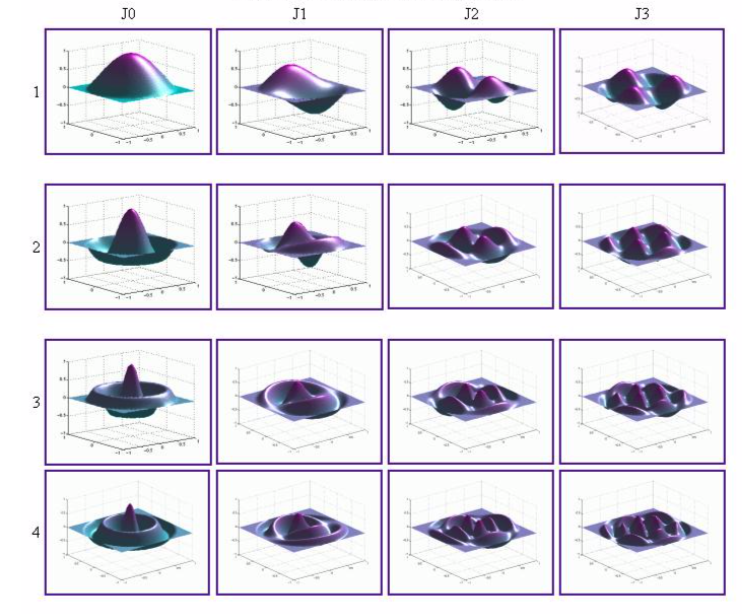
\includegraphics[scale=0.65]{Imagenes/Modos_Normales_Membrana_Circular.png}
\end{figure}
En el sitio \url{https://www.falstad.com/circosc/} verás una animación hecha en \texttt{java} (se conoce como applet) en donde se visualiza la vibración de la membrana circular. Es posible modificar el modo y frecuencia de oscilación, de tal manera que se muestra el cambio en la animación de la membrana.
\par
Desde el punto de vista computacional, es posible mostrar el resultado de la ED de Bessel para este ejemplo, pero toma en cuenta que la dificultad mayor es pasar de un dominio continuo (las soluciones de la ED) a un dominio discreto, dada la naturaleza del hardware, por lo que hay que hacer algunos ajustes en el algoritmo para que se resuelva la ecuación y se visualice el resultado.
\end{document}